\documentclass[a4paper]{article}
\usepackage{mystyle}

\begin{document}

\title{\citeauthor{Schrader2002Matlab} Roughness Model Analysis}
\author{Rodrigo García León\\
        M.Sc Student Human-Technology Interaction\\
        Department of Industrial Engineering \& Innovation Sciences\\
        Eindhoven University of Technology\\
        \texttt{r.garcia.leon@student.tue.nl}}

\maketitle

\section{Introduction} 

This document contains several notes regarding the implementation and the
obtained results of using the Roughness model implementation in MATLAB by
\citet{Schrader2002Matlab}. This implementation is based on the work of
\citet{Aures1985Ein} and \citet{Daniel1997Psychoacoustical}.

Furthermore, since the models of roughness and fluctuation strength are similar,
relevant details for the implementation of a fluctuation strength model will be
taken from the implementation of roughness model at hand.

\section{Implementation}

\subsection{Terhardt slopes stepness calculation}

Regarding the calculation of the steep of Terhardt slopes, a possible error was
detected in the source code. Listing \ref{lst:terhardt} shows the specific code
under questioning.

\lstinputlisting[
    style=MATLAB-editor,
    firstline=18,
    lastline=26,
    caption={Terhardt slopes steepness calculation},
    label={lst:terhardt}
]{/Users/rodrigo/Documents/MATLAB/Thesis/Roughness.m}

Line 5 of the code uses the expression
\lstinline[style=MATLAB-editor]!(230 / params.freqs(w))!, in which the variable
\lstinline[style=MATLAB-editor]!w! is used as index of the frequencies, instead
of \lstinline[style=MATLAB-editor]!whichL(w)!. Therefore it may be that the used
frequencies are not the correct ones, and errors might arise from this fact.

\section{Results}

In order to check the reliability of the results of the model implementation,
several plots from the original references were recreated. More specifically,
the upper left plots from Figure 3 \cite[pp.~118]{Daniel1997Psychoacoustical}
were made again. Two sets of plots were made, one were the original source code
was used (Figure \ref{fig:rwoc}), and another one were the correction to the
frequency indexes of Listing \ref{lst:terhardt} was used (Figure \ref{fig:rwc}).
From the graphs it can be seen that there is a difference of about 0.25 asper in
the values obtained. However, the uncorrected values are aligned with those
present in \citeauthor{Daniel1997Psychoacoustical} (Figure \ref{fig:rorigfig}).

\begin{figure}[ht]
    \centering
    \begin{minipage}[b]{0.45\linewidth}
        \centering
        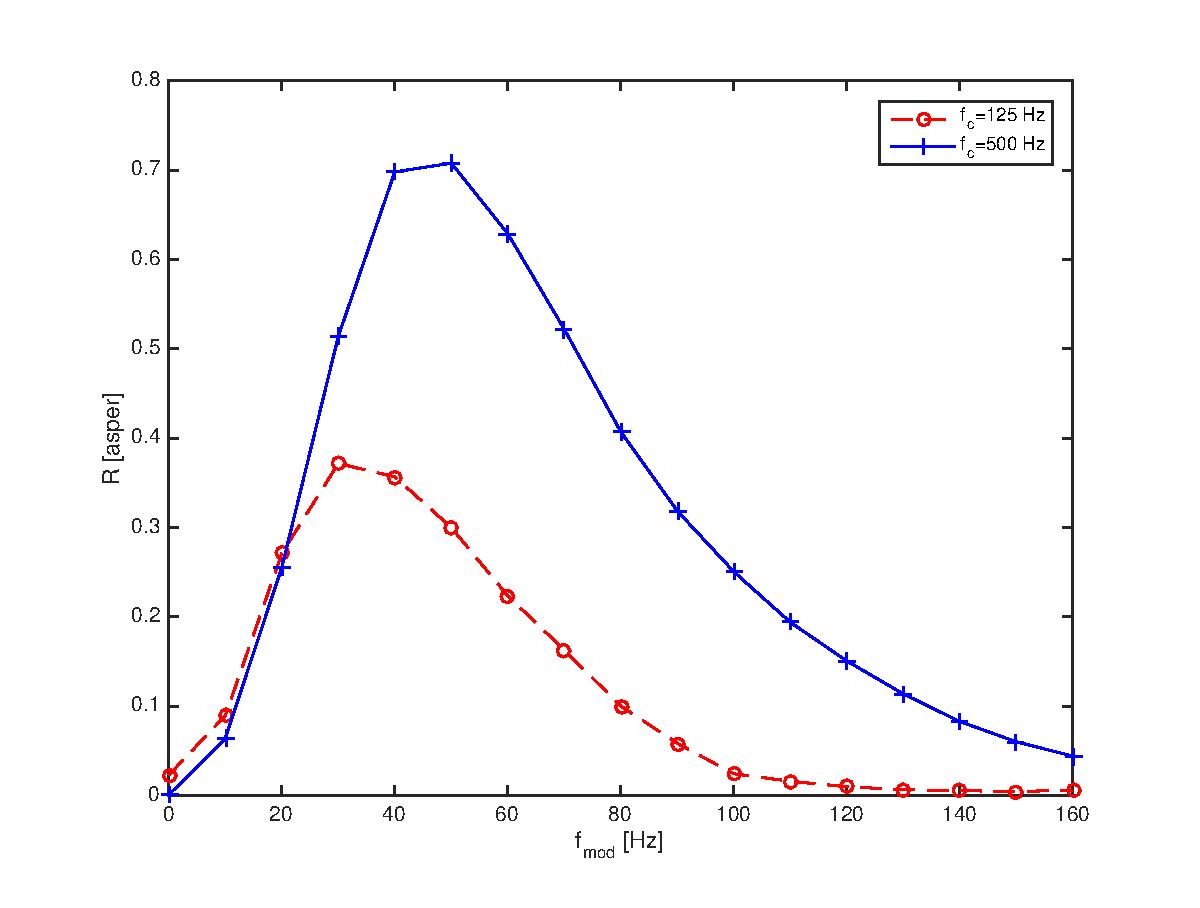
\includegraphics[height=5cm]
            {roughness-without-correction}
        \caption{Roughness without correction}
        \label{fig:rwoc}
    \end{minipage}
    \quad
    \begin{minipage}[b]{0.45\linewidth}
        \centering
        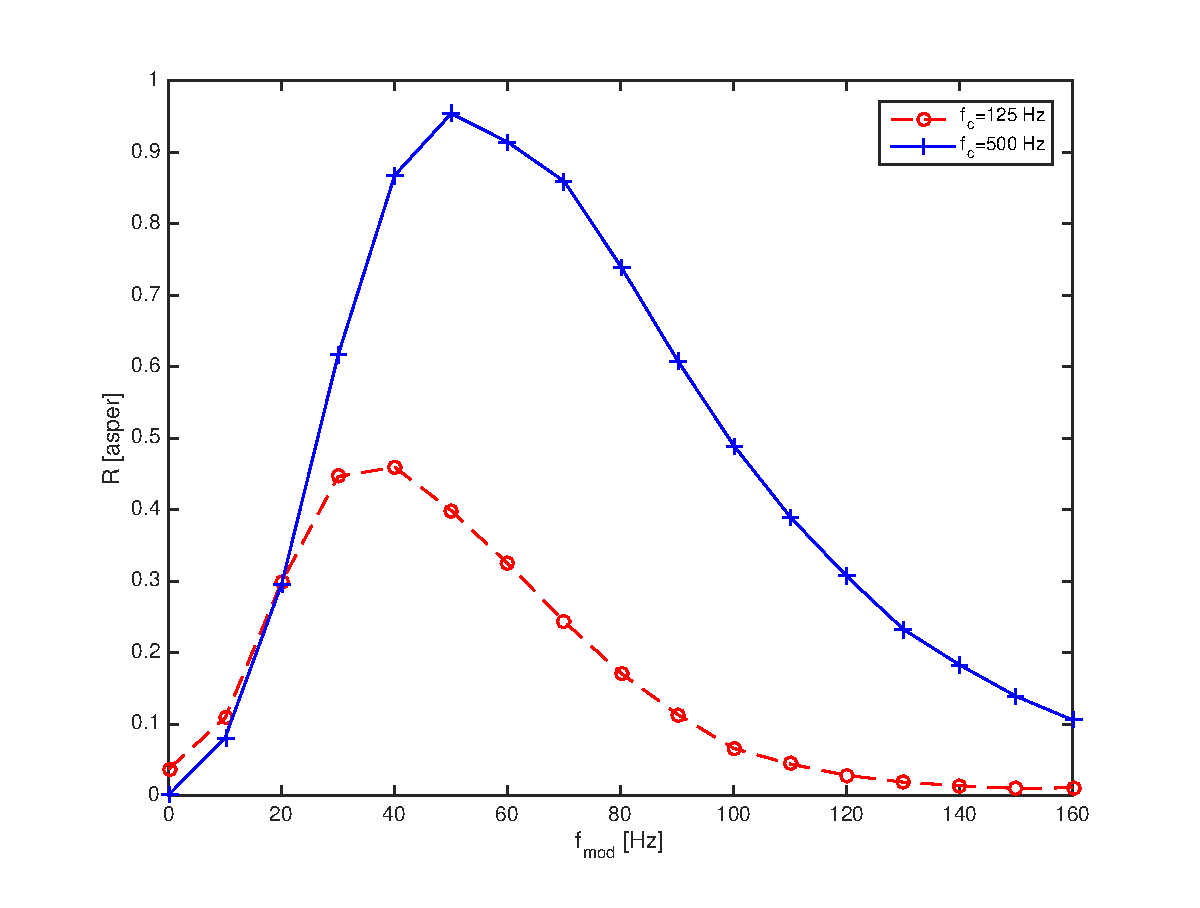
\includegraphics[height=5cm]
            {roughness-with-correction}
        \caption{Roughness with correction}
        \label{fig:rwc}
    \end{minipage}
\end{figure}

\begin{figure}[ht]
    \centering
    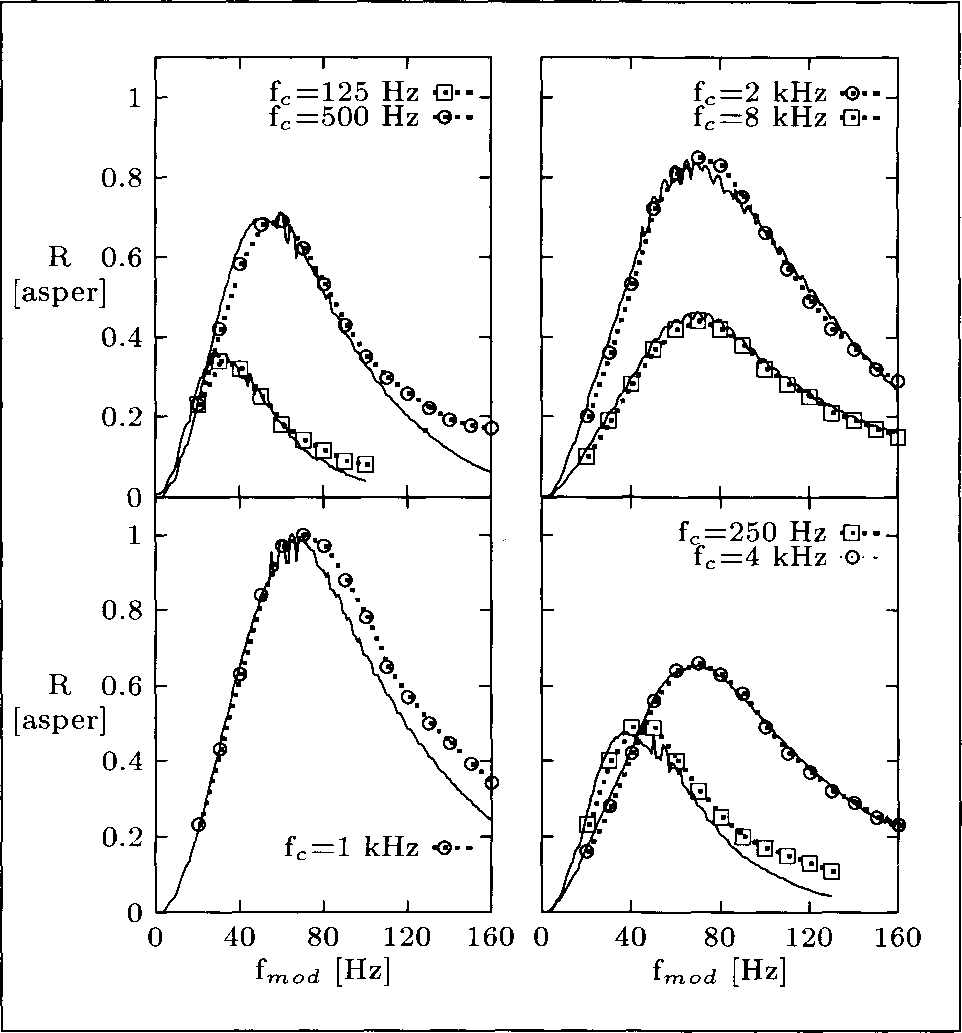
\includegraphics[height=8cm]{Daniel1997-RoughnessAMTones}
    \caption{Roughness of amplitude-modulates tones
        \cite[pp.~118]{Daniel1997Psychoacoustical}}
    \label{fig:rorigfig}
\end{figure}

\bibliographystyle{plainnat}
\bibliography{Remote}

\end{document}
